\chapter{Технологический раздел}
\section{Выбор и обоснование языка программирования}
Для реализации программы был выбран язык $C\verb|#|$ по нескольким причинам, среди которых возможность создания настольных приложений с использованием $Windows Forms$, интеграция с $.NET~Framework$, что обеспечивает высокую производительность и безопасность приложений, и поддержка объектно-ориентированного программирования.
\section{Хранение и обмен данными в системе}
Диаграмма классов представлена на рисунке~\ref{fig:class_diagram}. Математическая модель выбранная для пузырьков представлена в программе классом $Bubble$, являющимся потомком класса $Obj$. Также от класса $Obj$ наследуется класс $CombinedBubble$, то есть пузырьковый кластер. 

Объекты класса $Contour$ используются для отражения перемещения пузырьков и пузырьковых кластеров, без постоянной перерисовки трёхмерной сцены с использованием алгоритма обратной трассировки лучей.

Класс $Form1$ представляет собой основное окно пользовательского интерфейса приложения, именно в нём обрабатываются все события связанные с элементами управления.

Важно упомянуть, тип данных, характерный для $C\verb|#|$ и являющийся частью почти всех классов данной программы, -- $Vector3D$~\cite{vector3d}. Это структура, имеющая три поля, которые могут соответствовать координатам в пространстве, и все основные методы, нужные для работы с координатами или векторами. 
\begin{figure}[h]
	\centering
	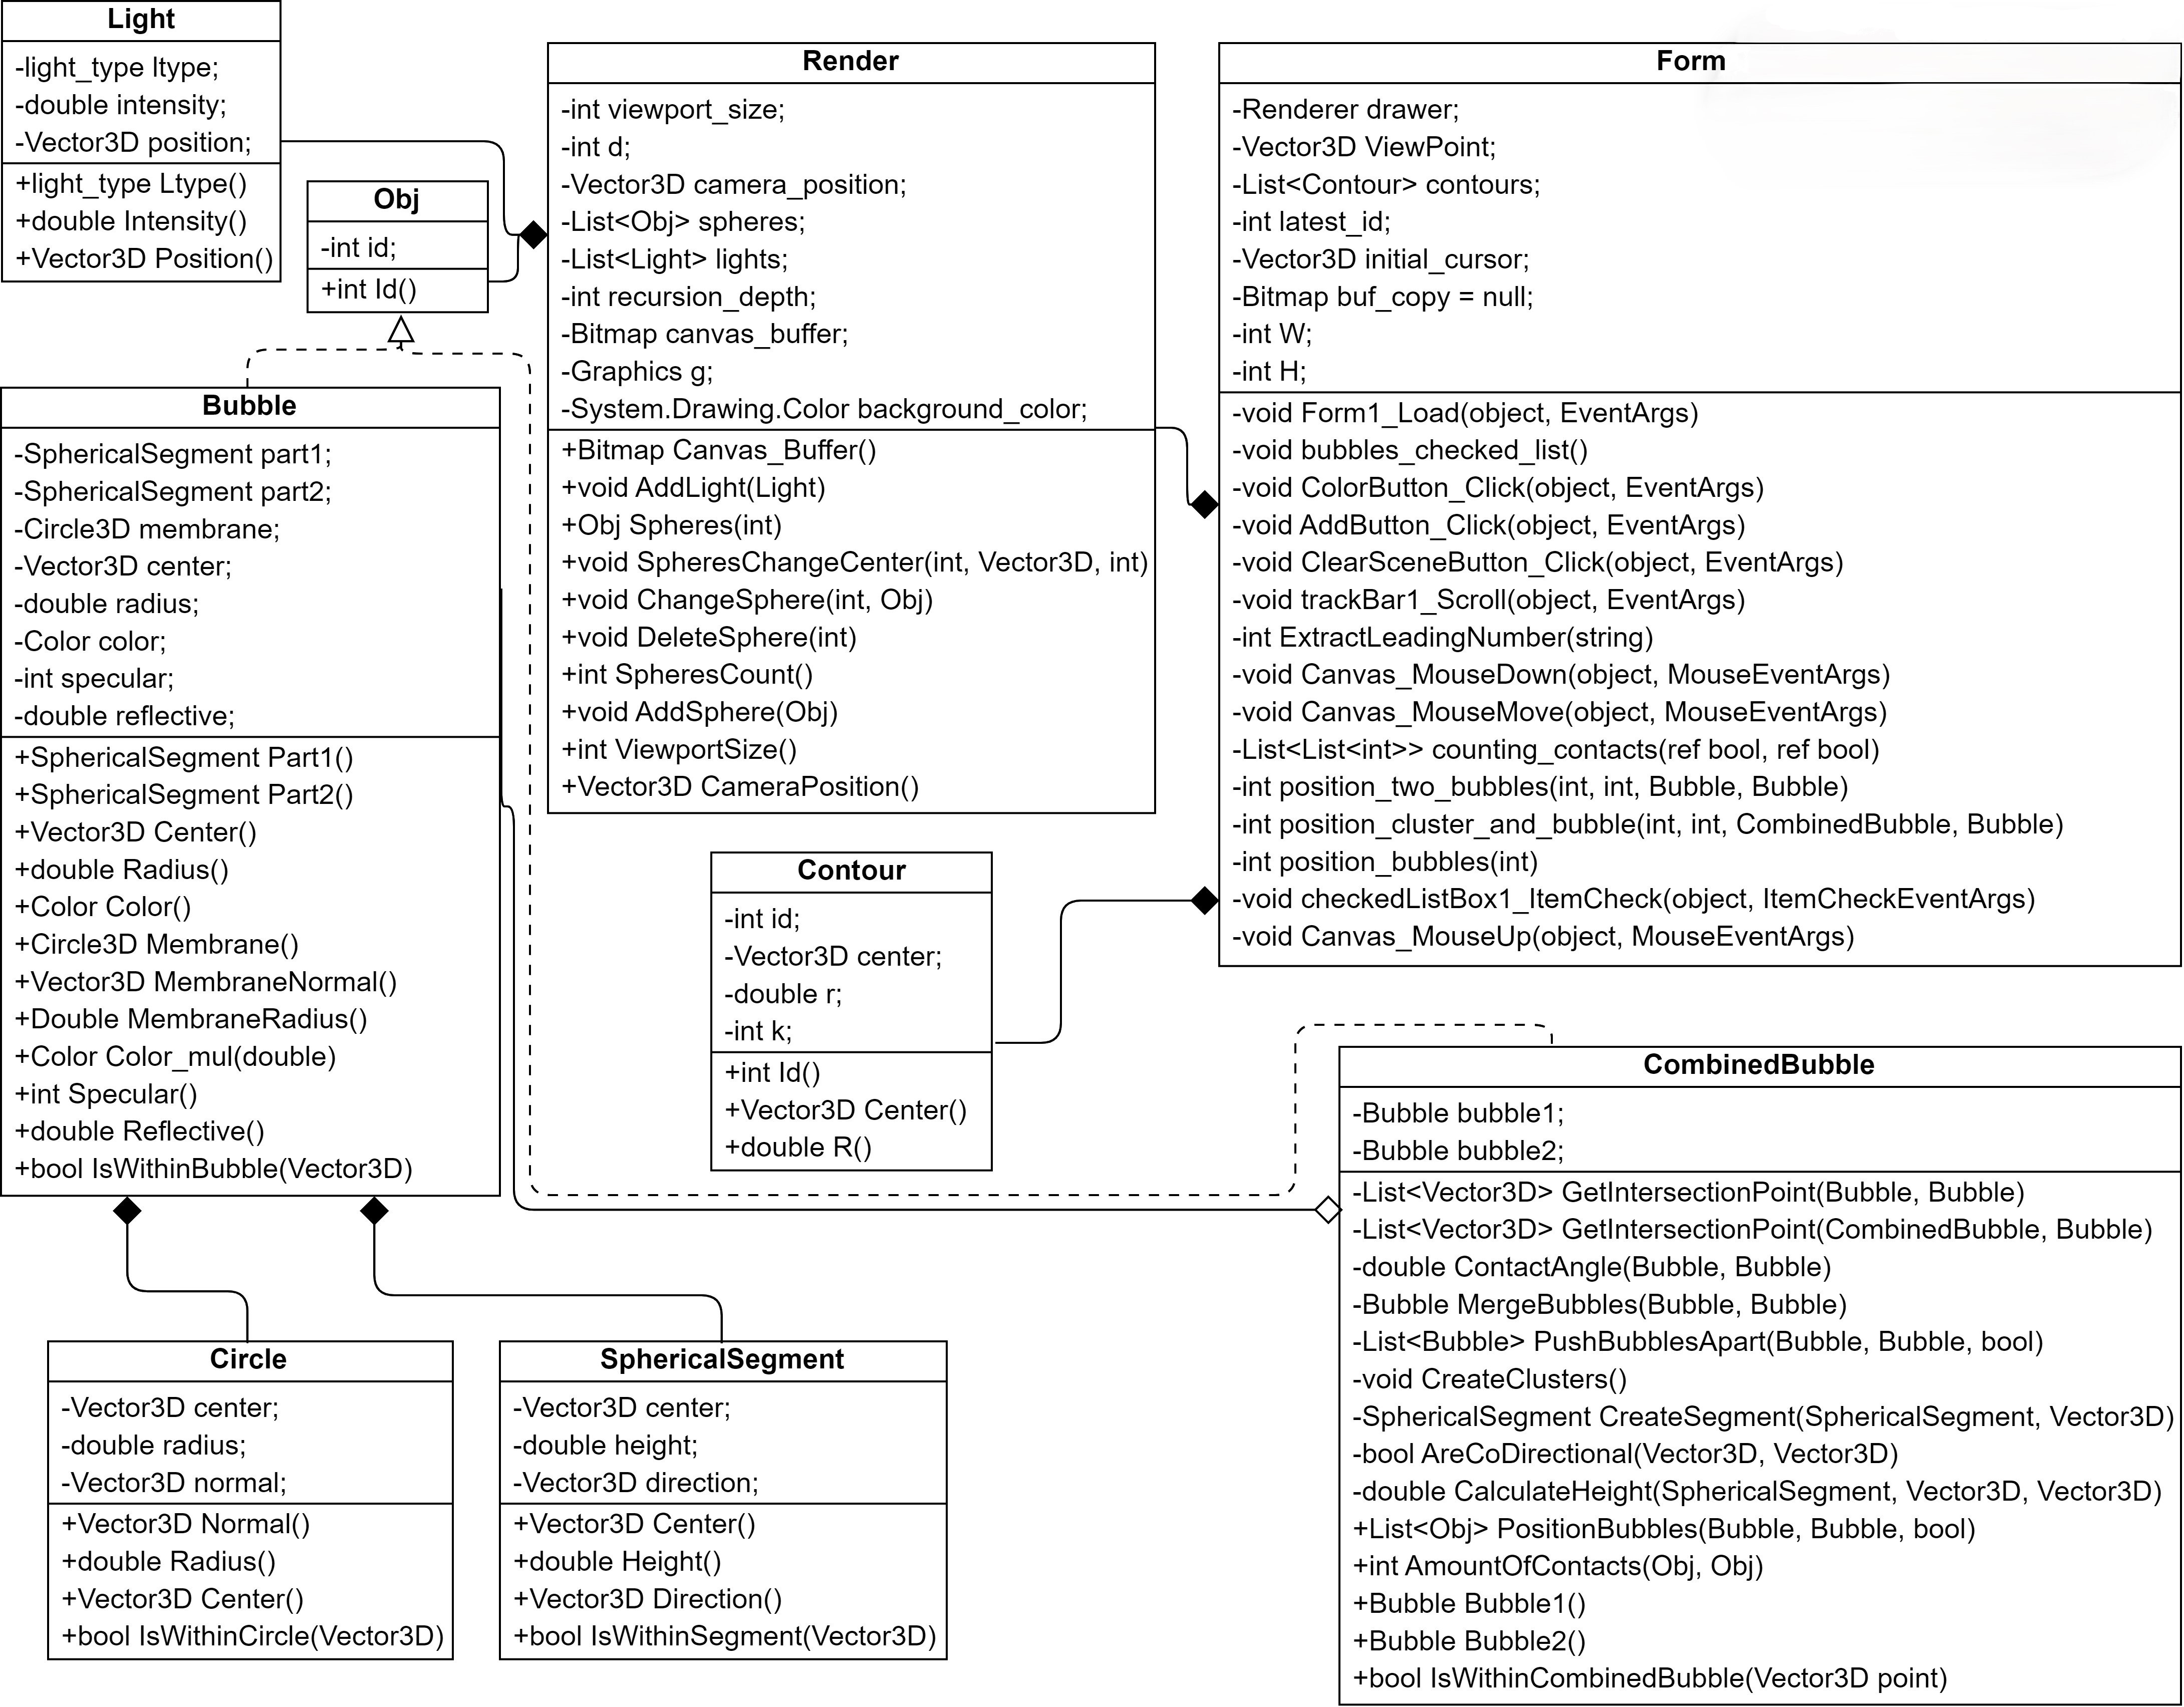
\includegraphics[angle=90, width=1\linewidth]{pictures/КГ_курсач_диаграмма классов.jpg}
	\caption{Диаграмма классов}
	\label{fig:class_diagram}
\end{figure}
\clearpage

\section{Интерфейс пользователя}
На рисунке~\ref{fig:interface} представлен пользовательский интерфейс. Ось $ox$ направлена вправо, $oy$ -- вверх, $oz$ -- от пользователя. Подробнее:
\begin{enumerate}[label={\arabic*)}]
	\item блок, позволяющий добавить на сцену ещё один пузырёк (можно указать координаты центра в пространстве, радиус и цвет);
	\item элемент управления, позволяющий приблизить или удалить камеру от объектов на сцене, вдоль оси $oz$;
	\item список объектов, присутствующих на сцене (при выборе элемента в этом блоке, его можно будет перемещать по сцене);
	\item кнопка отчистки сцены;
	\item сцена.  
	
\end{enumerate}
\begin{figure}[h]
	\centering
	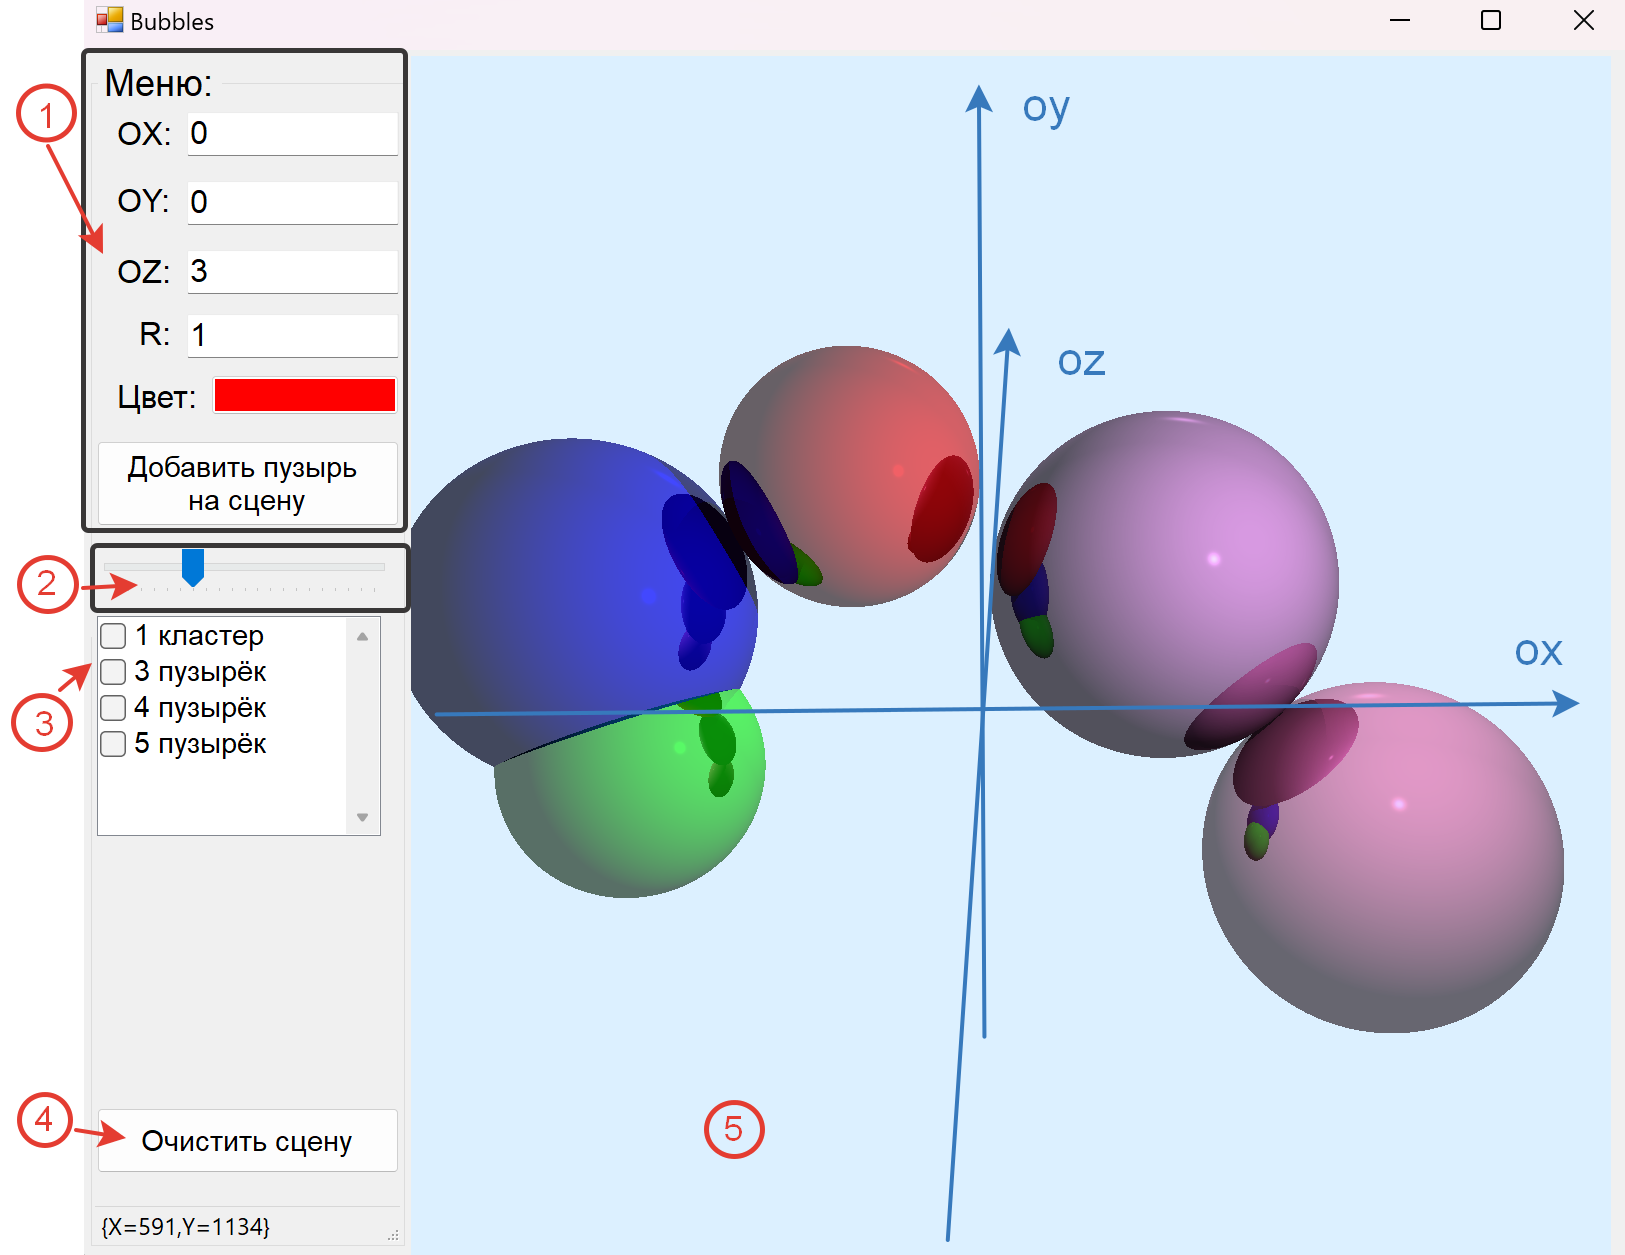
\includegraphics[width=1\linewidth]{pictures/interface.png}
	\caption{Интерфейс пользователя}
	\label{fig:interface}
\end{figure}

\section{Сообщения системы}

Если после перемещения или создания пузырь будет иметь более чем одно пересечение с другими пузырями на сцене, будет выведено сообщение об ошибке "Больше чем одно пересечение".

Если после перемещения или создания пузырь с одним из пузырей какого-либо кластера будет иметь предполагающий образование кластера, будет выведено сообщение об ошибке "Угол соприкосновения принадлежит [55, 65]. Невозможно образование кластера из трёх пузырей".

\section{Функциональное тестирование}
\begin{figure}[h]
	\centering
	\begin{subfigure}{0.45\textwidth}
		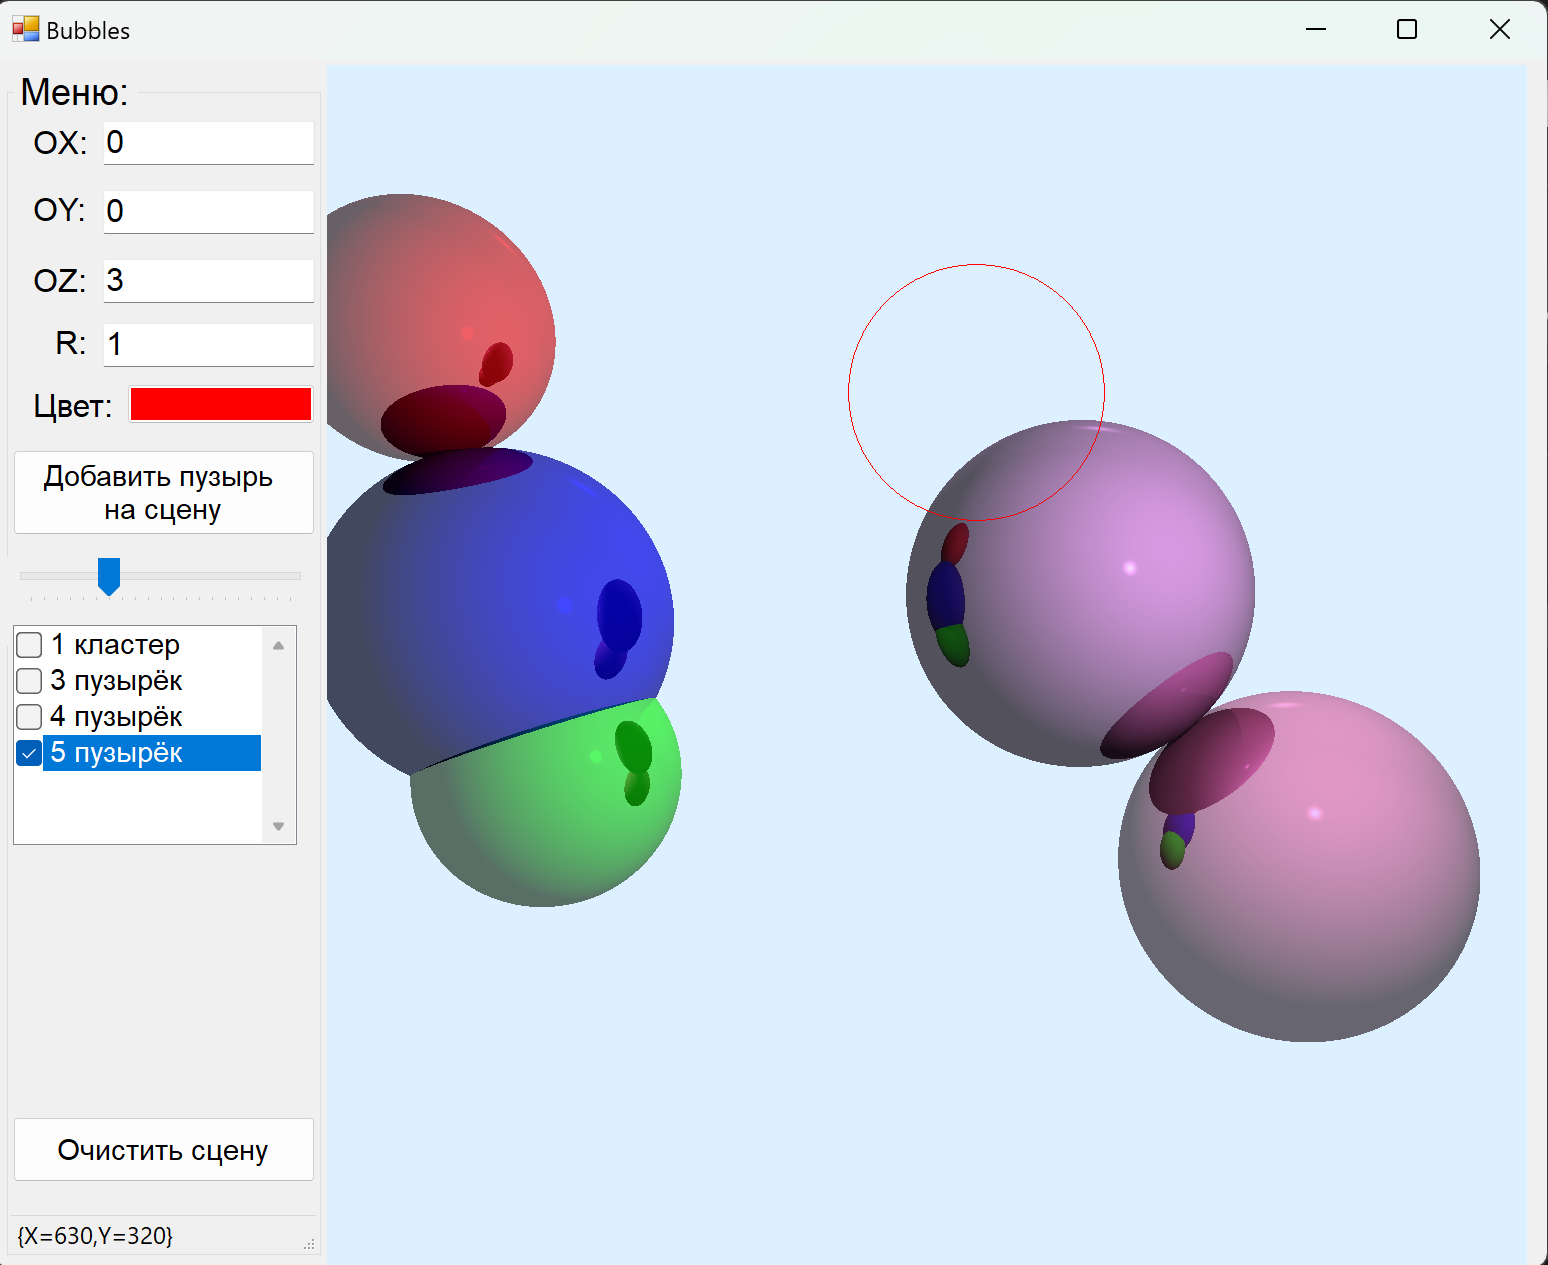
\includegraphics[width=\linewidth]{pictures/test1_1.png}
		\caption{До преобразования}
		\label{fig:1first}
	\end{subfigure}
	\hfill
	\begin{subfigure}{0.45\textwidth}
		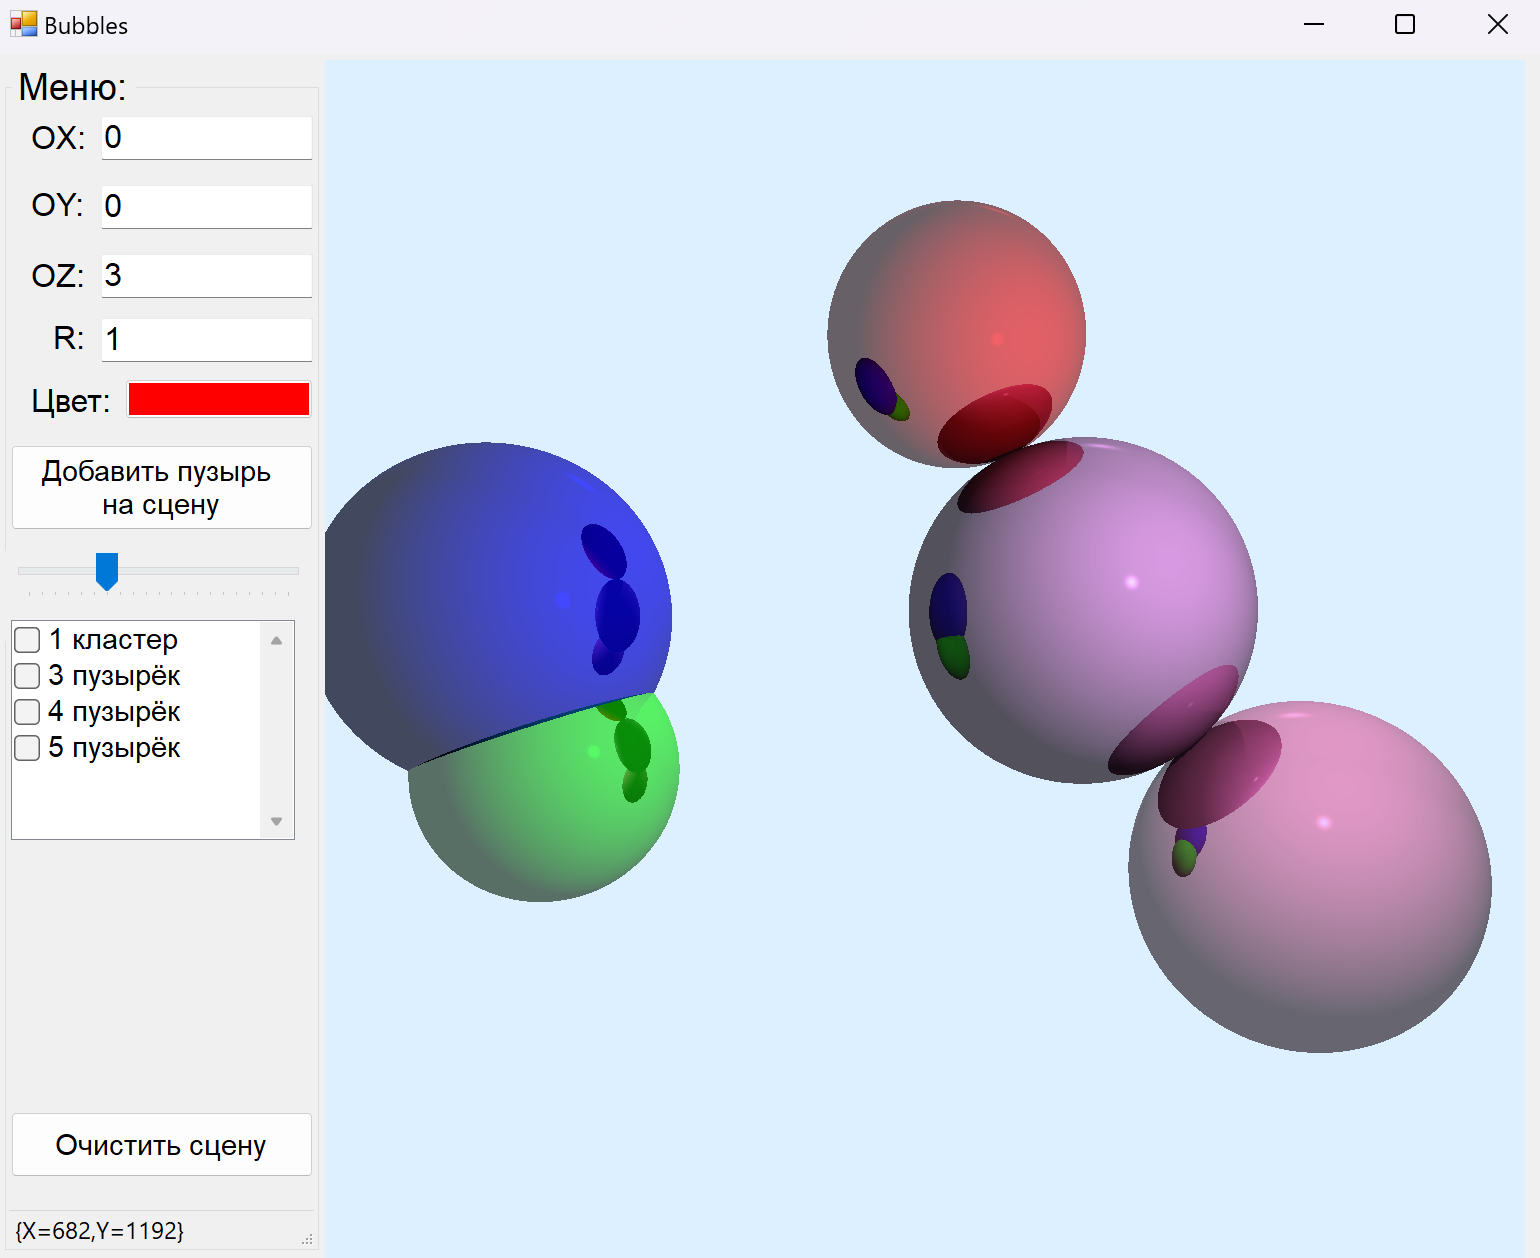
\includegraphics[width=\linewidth]{pictures/test1_2.png}
		\caption{После преобразования}
		\label{fig:1second}
	\end{subfigure}
	\caption{Тест №1: отталкивание}
	\label{fig:test1}
\end{figure}
\begin{figure}[h]
	\centering
	\begin{subfigure}{0.45\textwidth}
		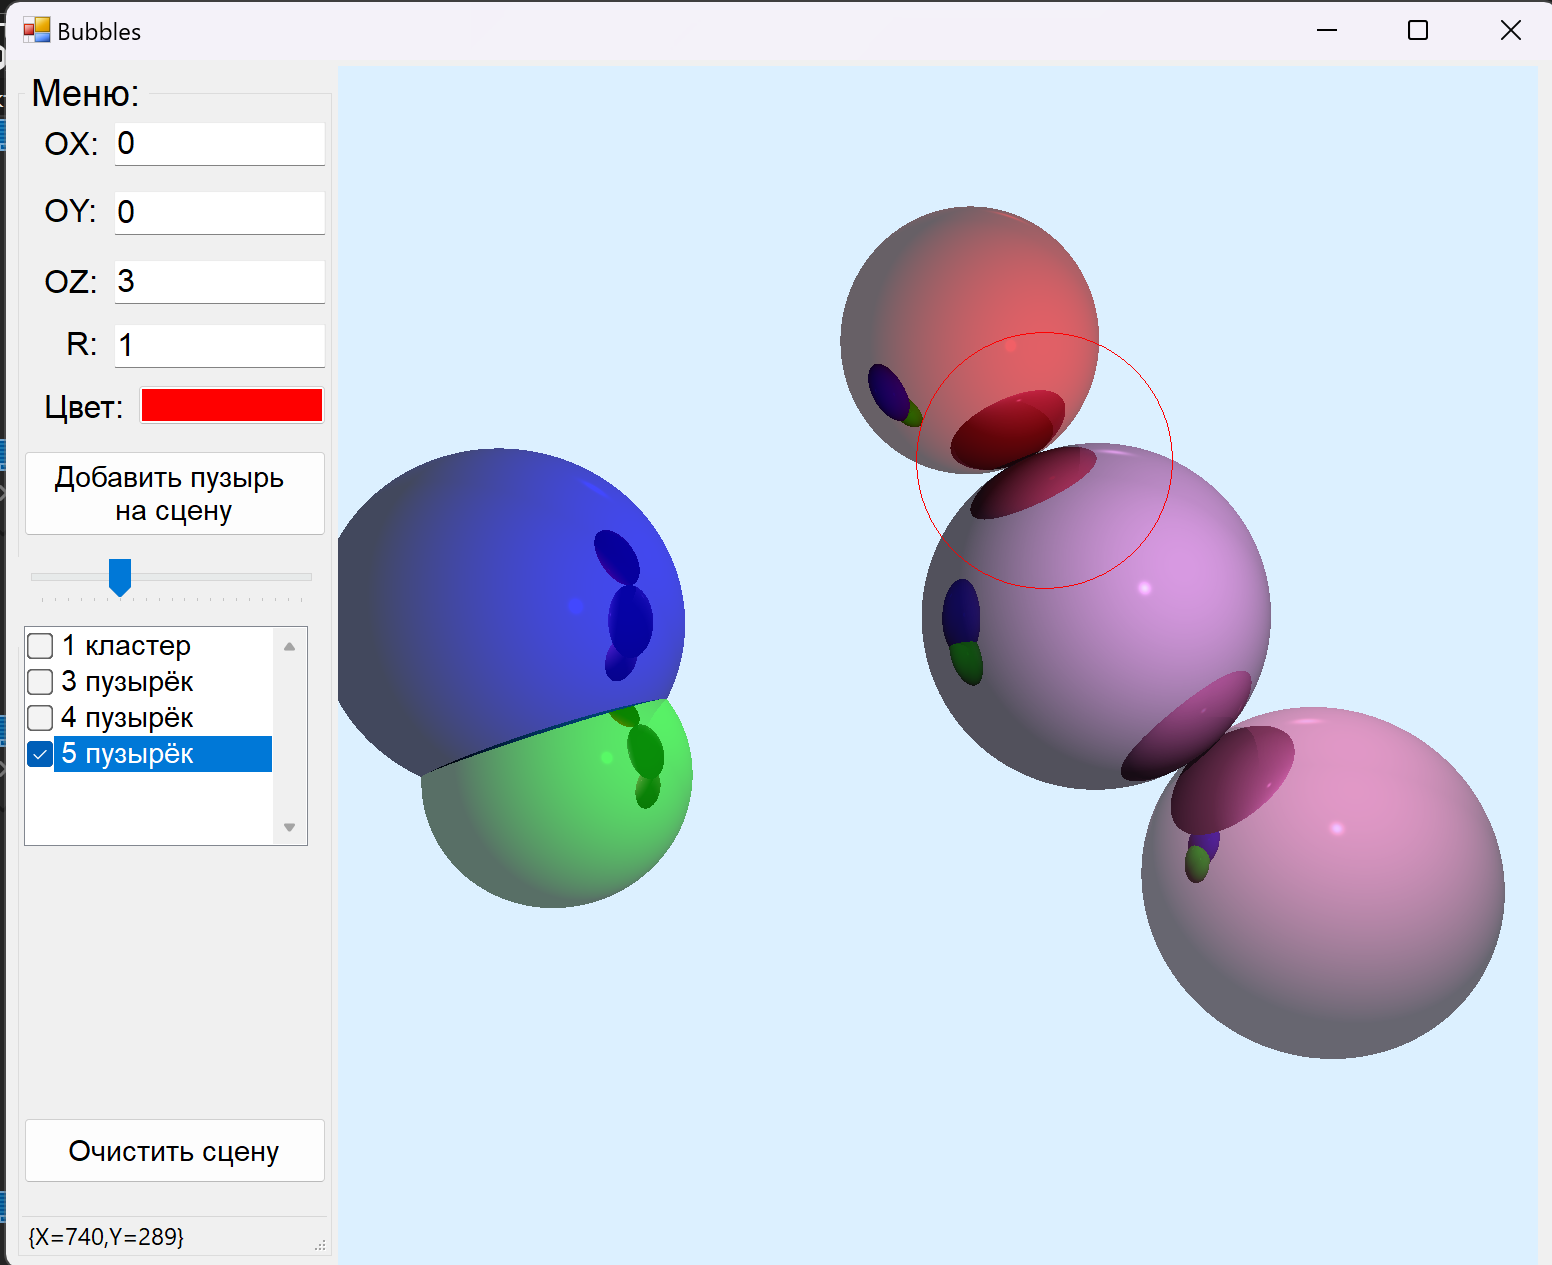
\includegraphics[width=\linewidth]{pictures/test2_1.png}
		\caption{До преобразования}
		\label{fig:2first}
	\end{subfigure}
	\hfill
	\begin{subfigure}{0.45\textwidth}
		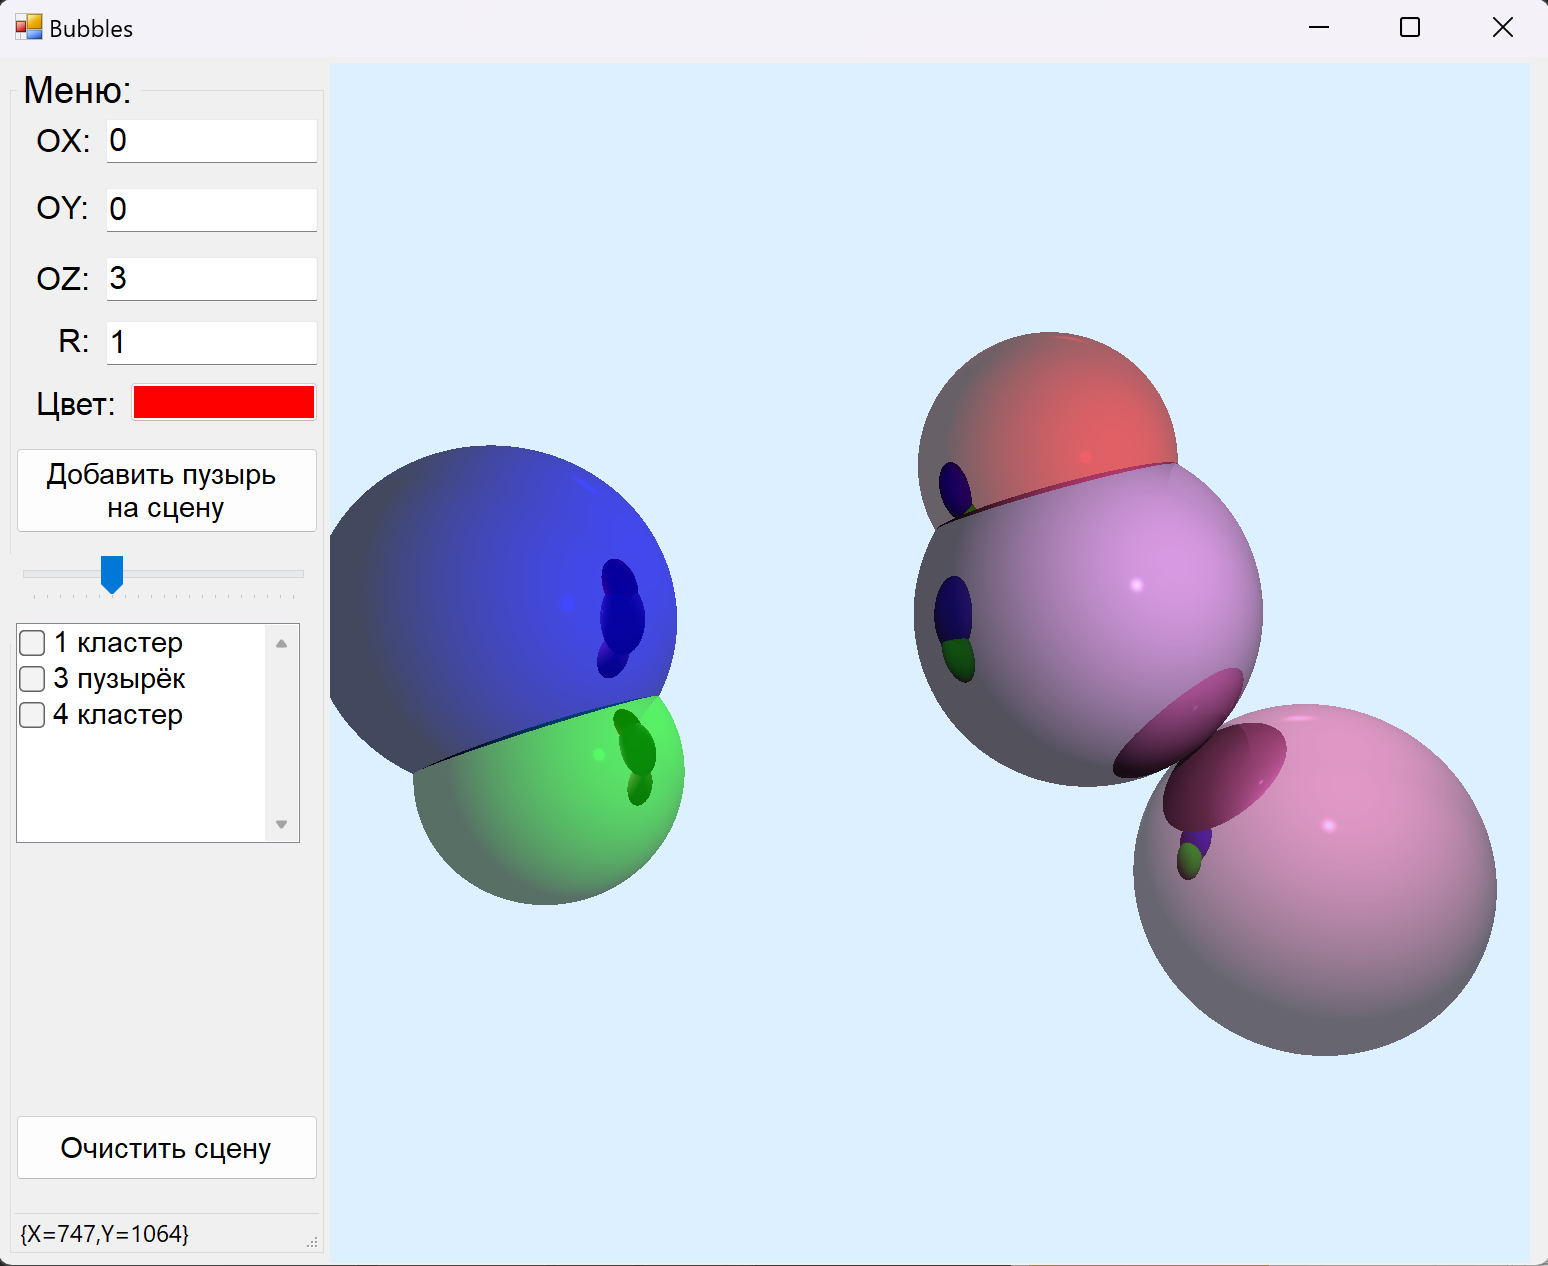
\includegraphics[width=\linewidth]{pictures/test2_2.png}
		\caption{После преобразования}
		\label{fig:2second}
	\end{subfigure}
	\caption{Тест №2: образование кластера}
	\label{fig:test2}
\end{figure}
\begin{figure}[h]
	\centering
	\begin{subfigure}{0.45\textwidth}
		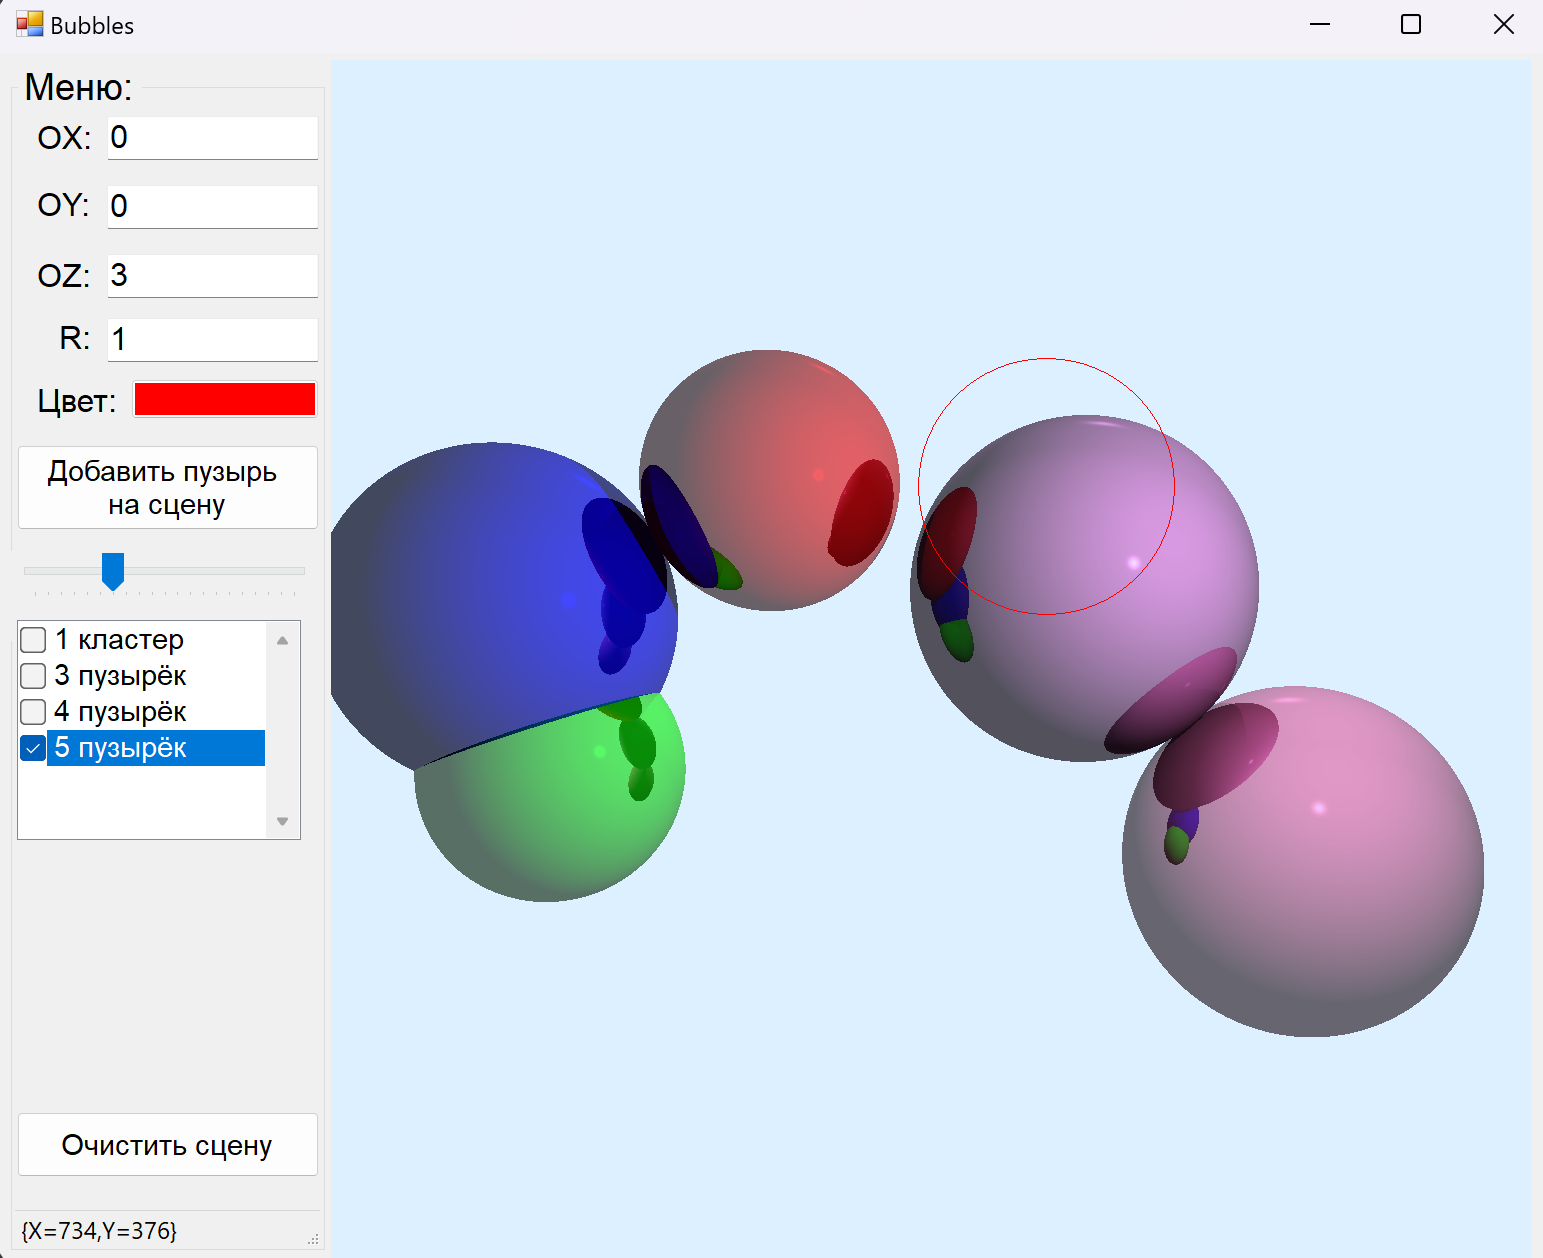
\includegraphics[width=\linewidth]{pictures/test3_1.png}
		\caption{До преобразования}
		\label{fig:3first}
	\end{subfigure}
	\hfill
	\begin{subfigure}{0.45\textwidth}
		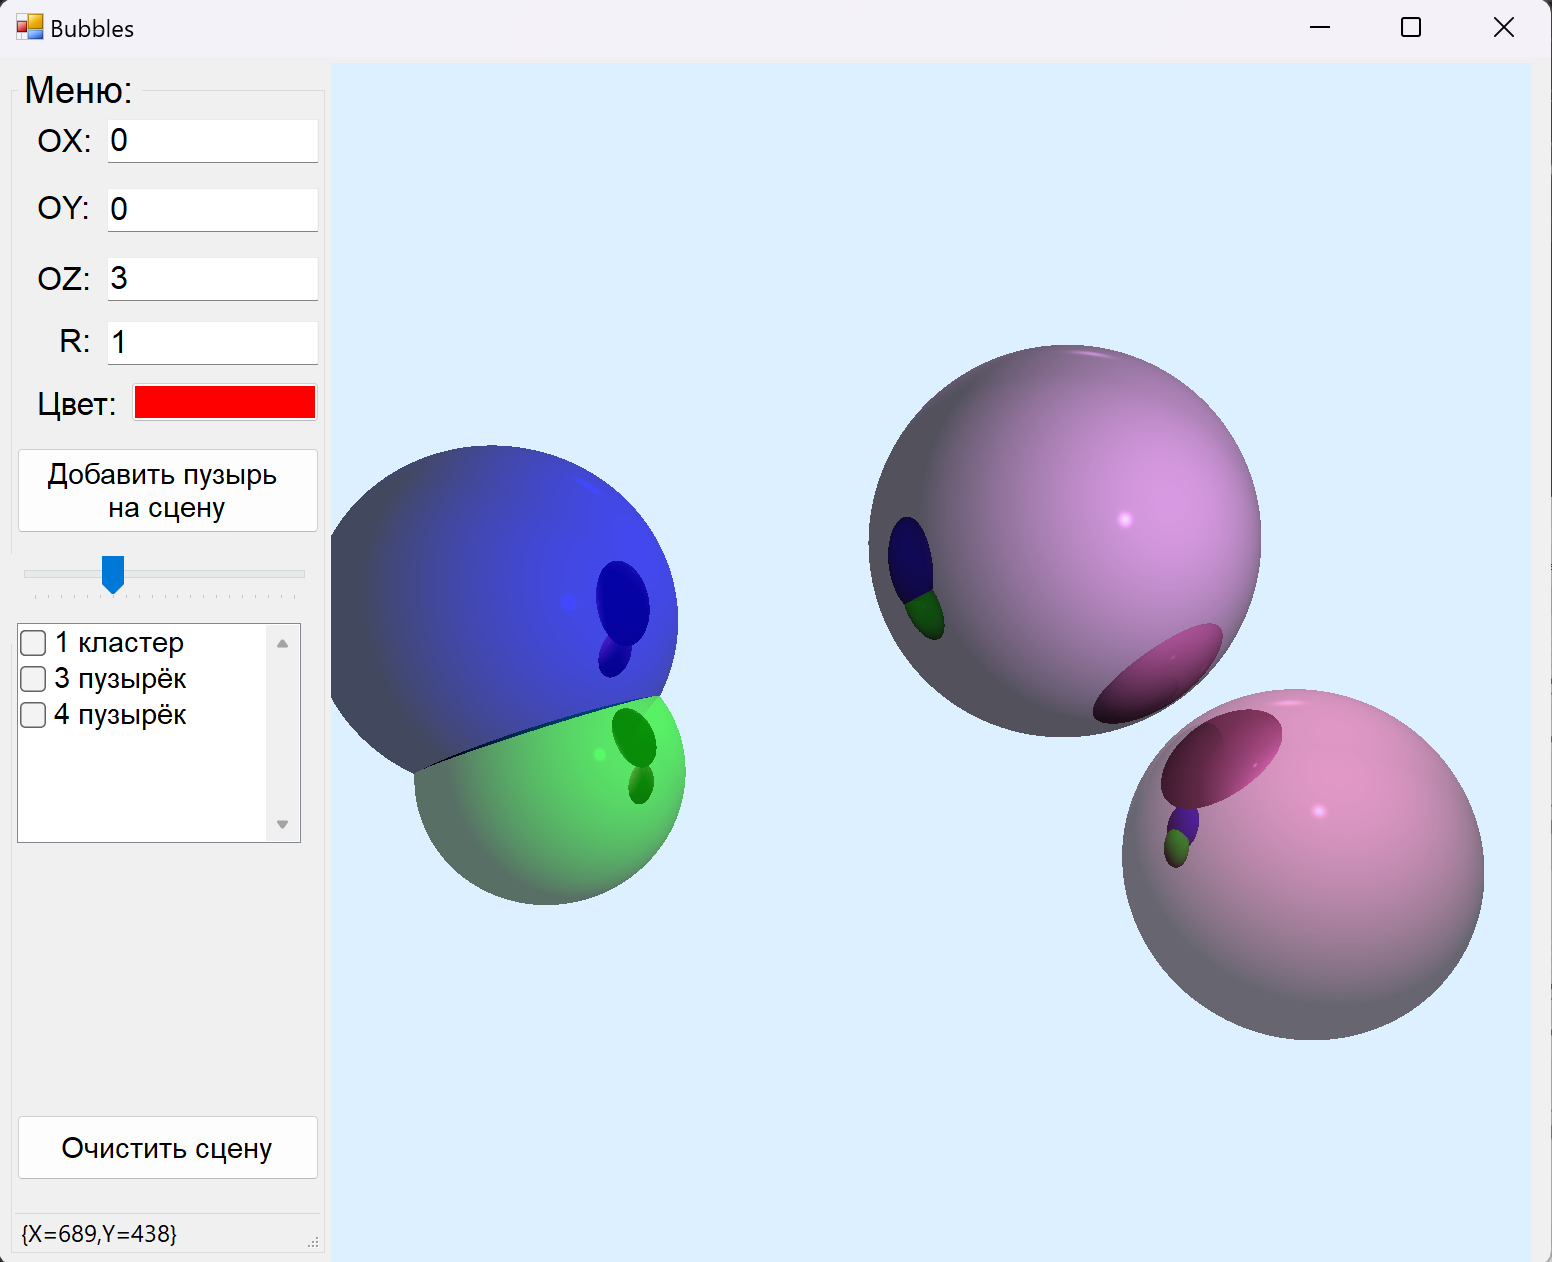
\includegraphics[width=\linewidth]{pictures/test3_2.png}
		\caption{После преобразования}
		\label{fig:3second}
	\end{subfigure}
	\caption{Тест №3: слияние}
	\label{fig:test3}
\end{figure}
\begin{figure}[h]
	\centering
	\begin{subfigure}{0.45\textwidth}
		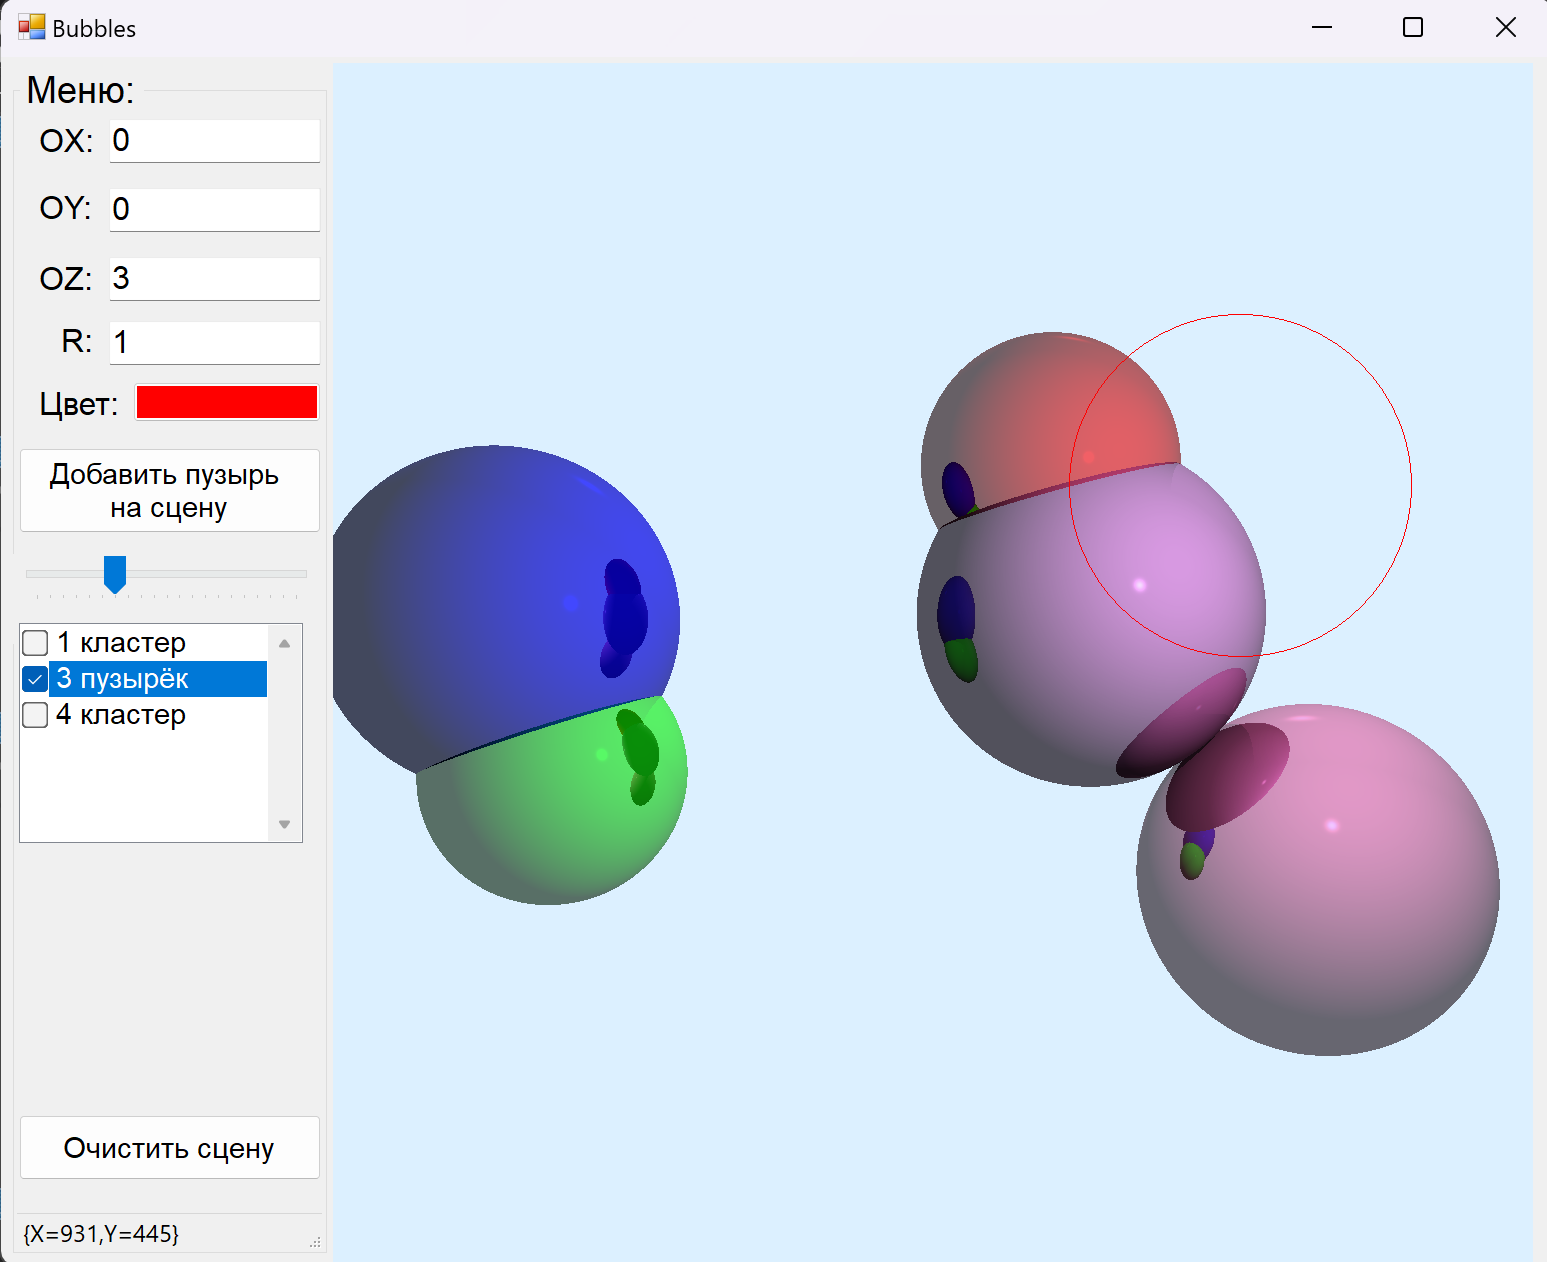
\includegraphics[width=\linewidth]{pictures/test4_1.png}
		\caption{До преобразования}
		\label{fig:4first}
	\end{subfigure}
	\hfill
	\begin{subfigure}{0.45\textwidth}
		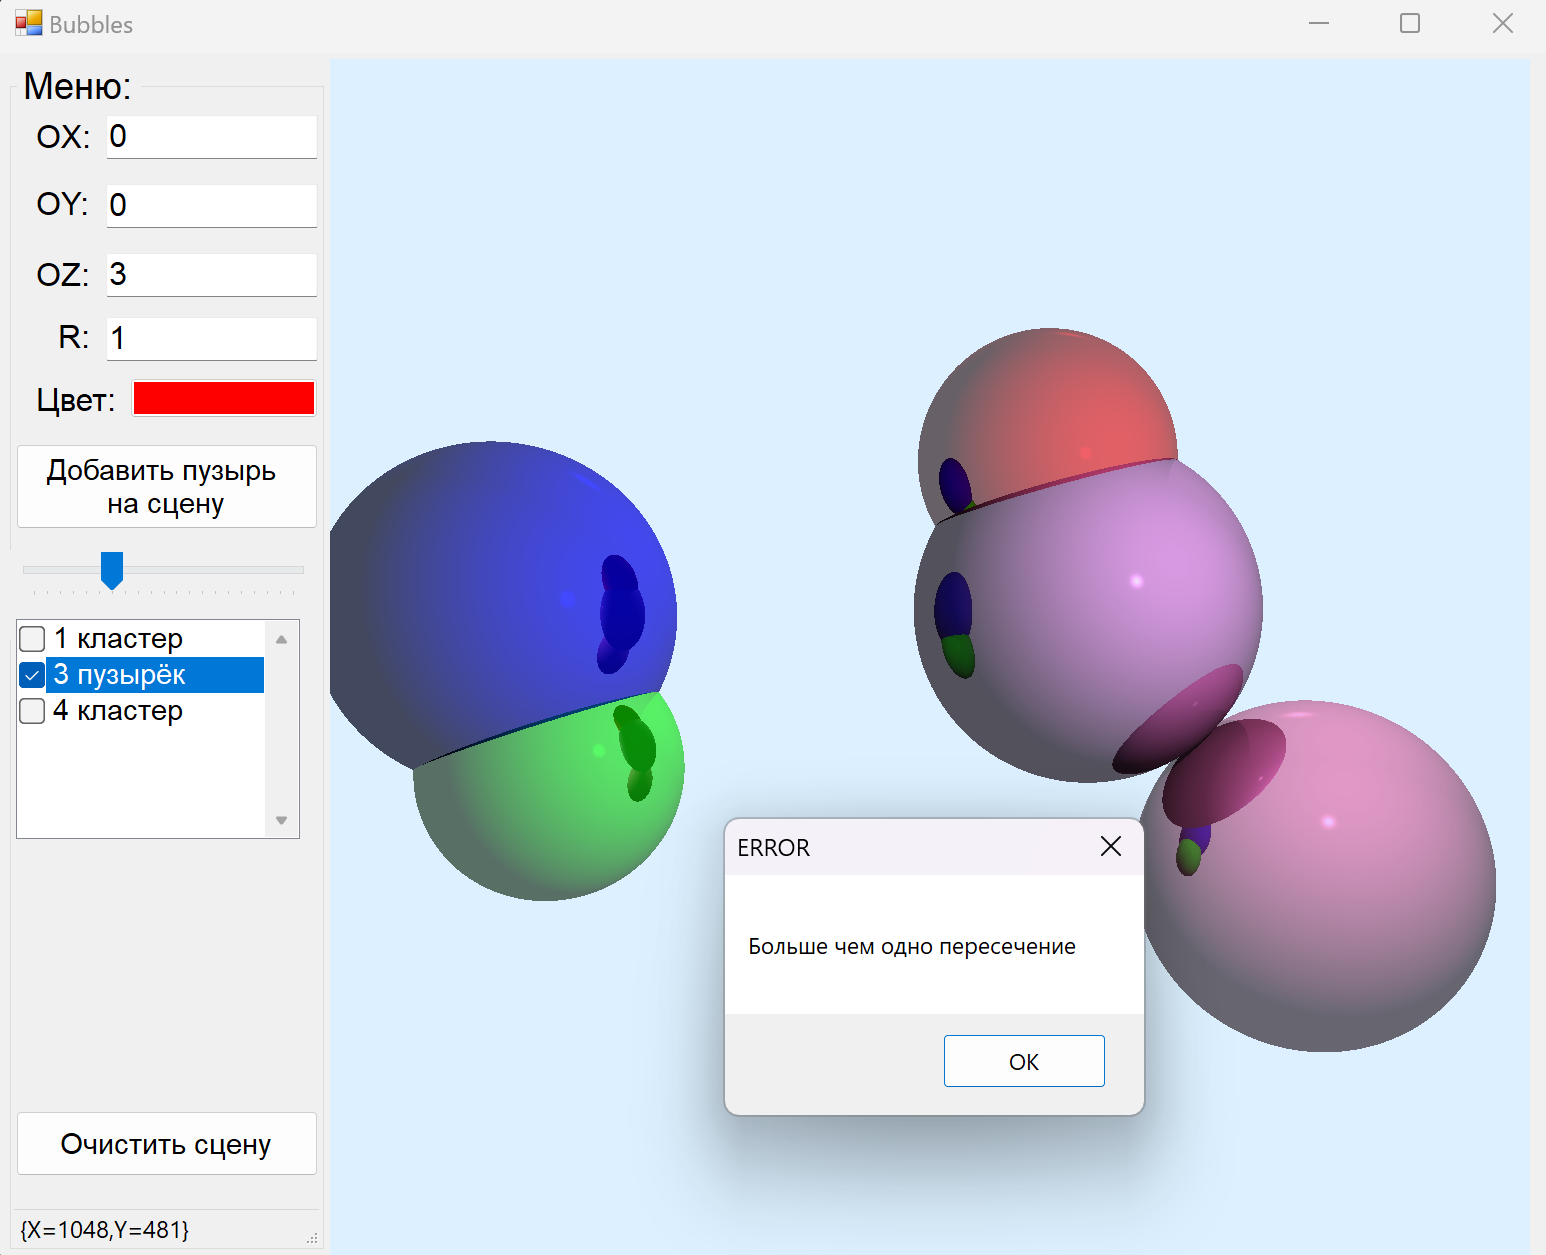
\includegraphics[width=\linewidth]{pictures/test4_2.png}
		\caption{После преобразования}
		\label{fig:4second}
	\end{subfigure}
	\caption{Тест №4: больше чем одно пересечение}
	\label{fig:test4}
\end{figure}
\begin{figure}[h]
	\centering
	\begin{subfigure}{0.45\textwidth}
		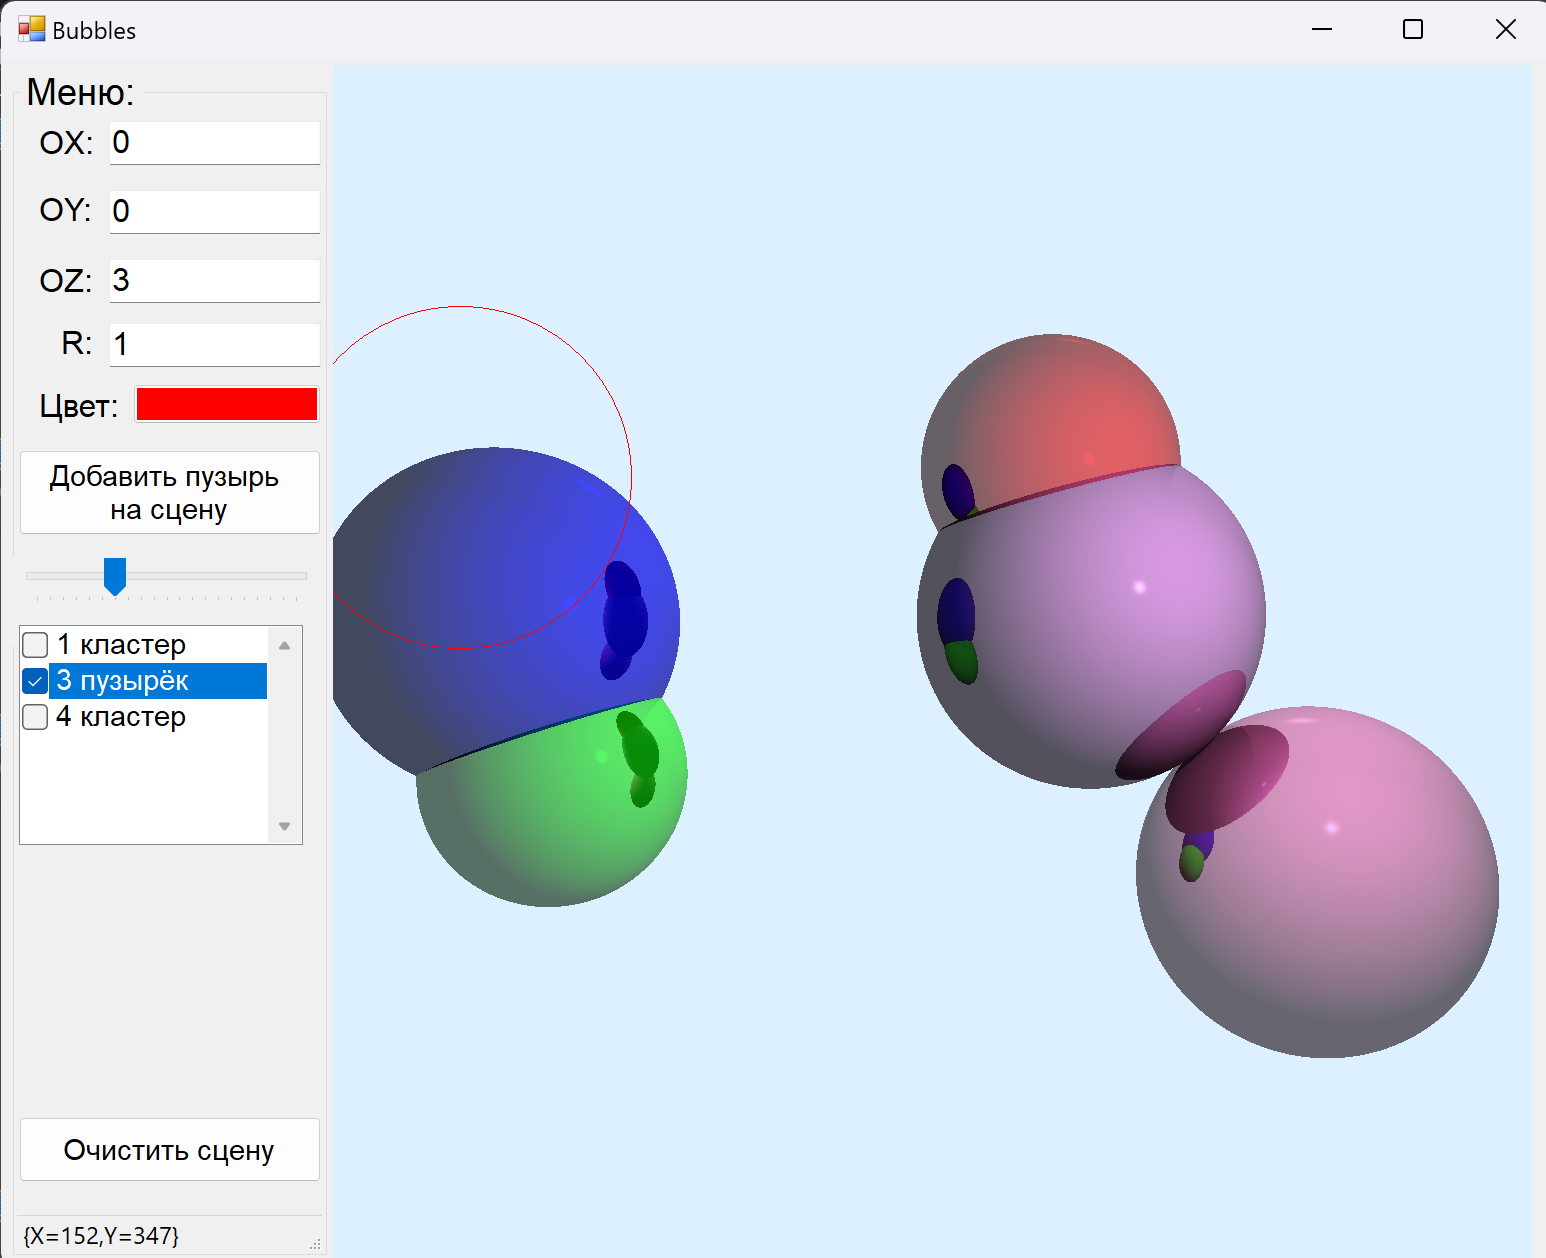
\includegraphics[width=\linewidth]{pictures/test5_1.png}
		\caption{До преобразования}
		\label{fig:5first}
	\end{subfigure}
	\hfill
	\begin{subfigure}{0.45\textwidth}
		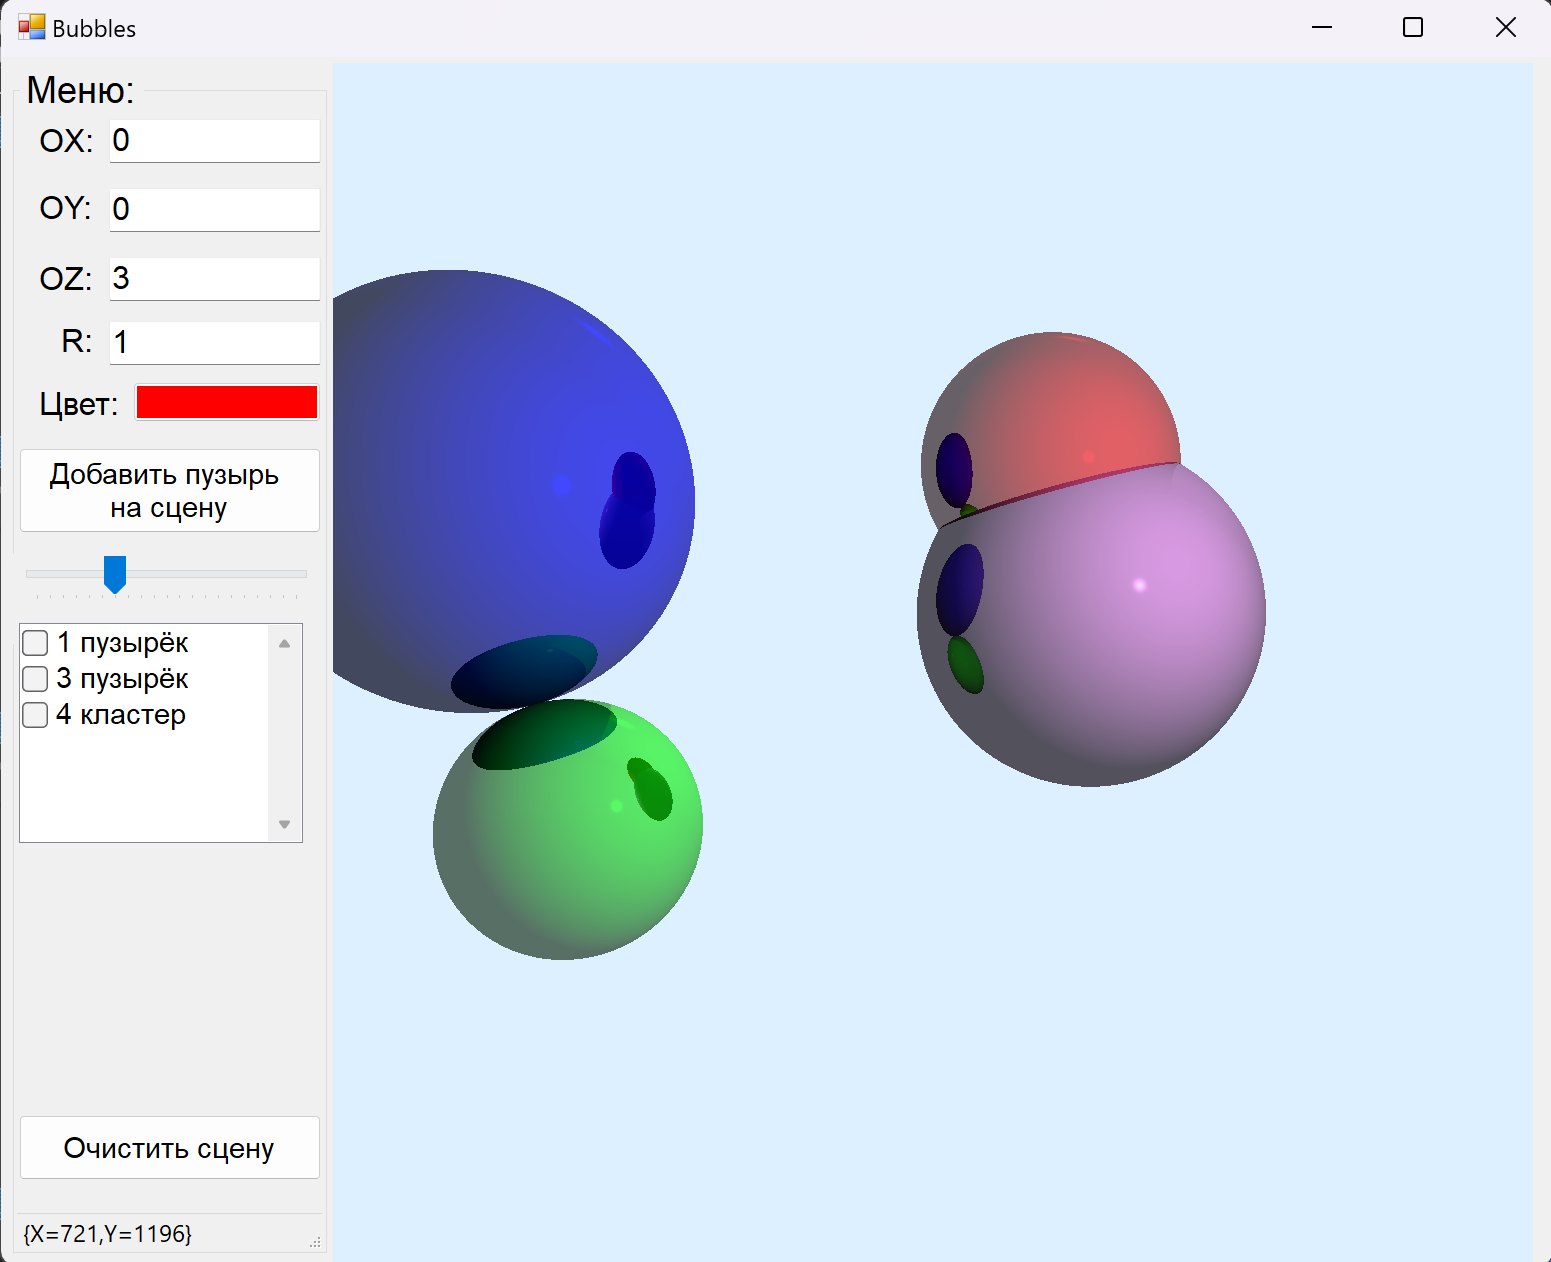
\includegraphics[width=\linewidth]{pictures/test5_2.png}
		\caption{После преобразования}
		\label{fig:5second}
	\end{subfigure}
	\caption{Тест №5: слияние с частью кластера}
	\label{fig:test5}
\end{figure}
\begin{figure}[h]
	\centering
	\begin{subfigure}{0.45\textwidth}
		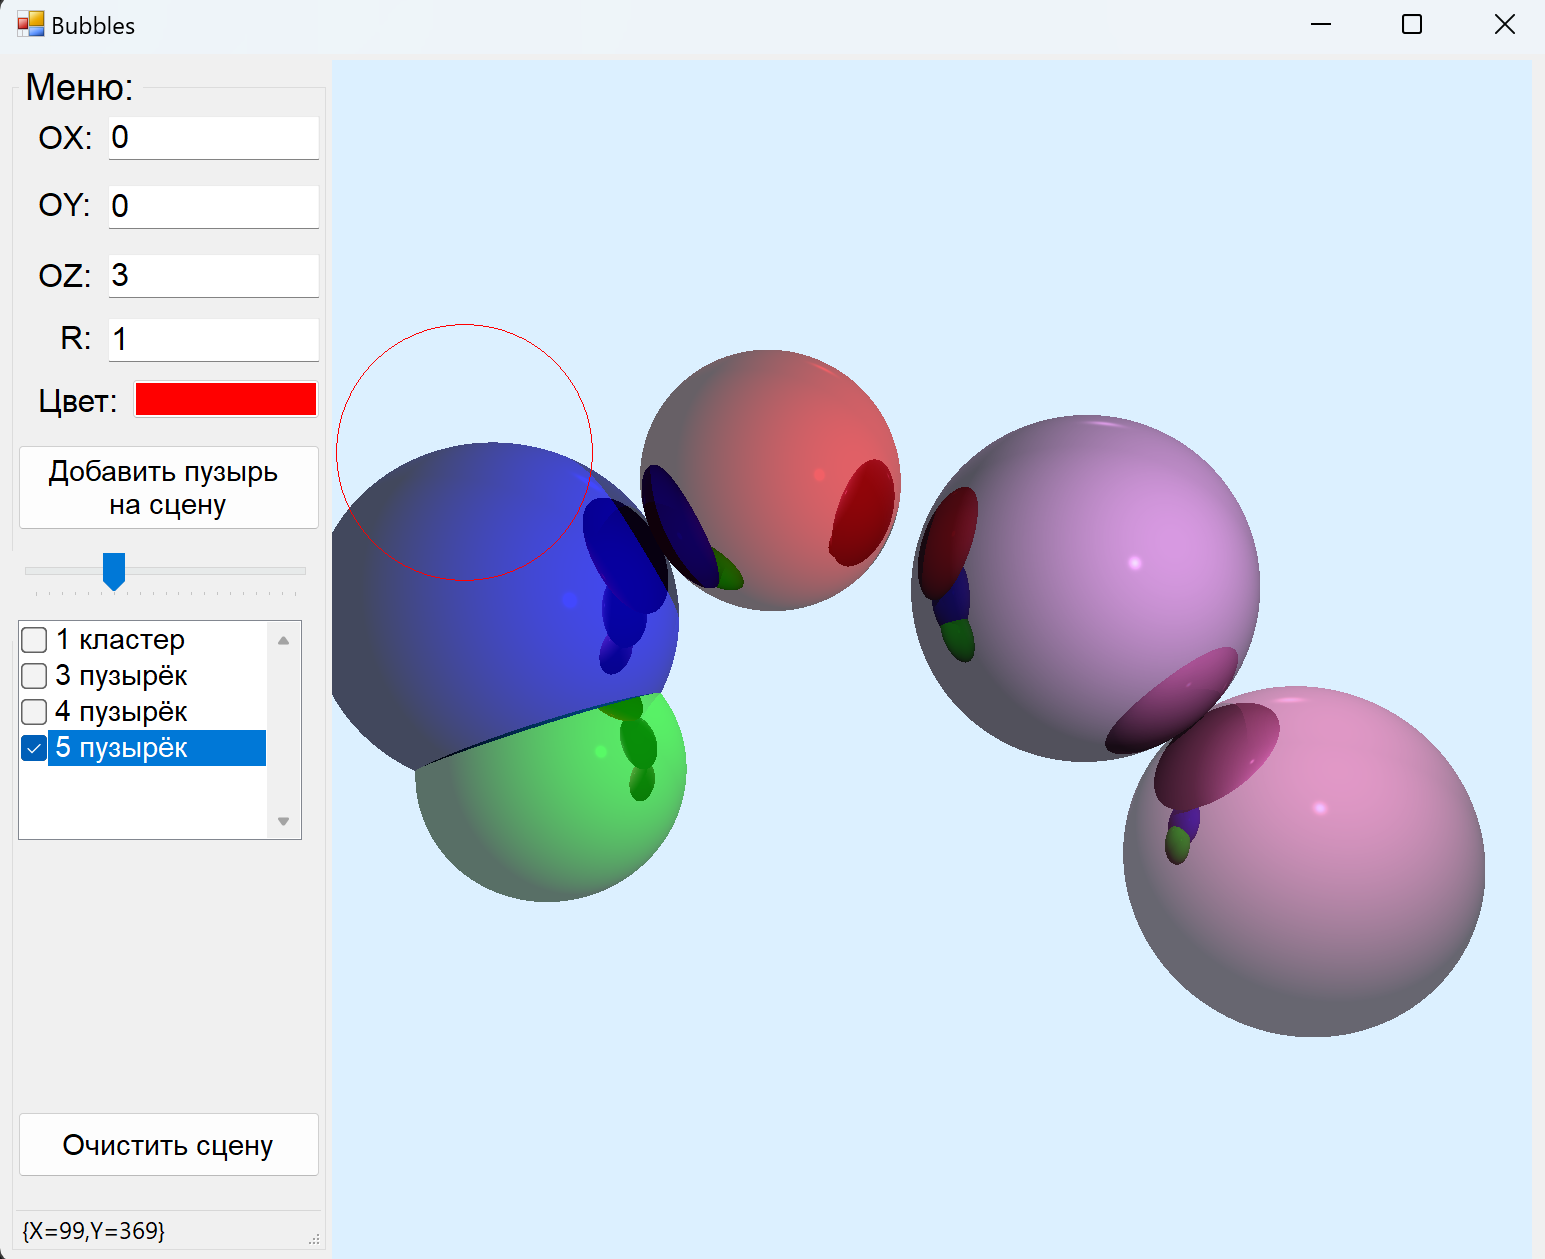
\includegraphics[width=\linewidth]{pictures/test6_1.png}
		\caption{До преобразования}
		\label{fig:6first}
	\end{subfigure}
	\hfill
	\begin{subfigure}{0.45\textwidth}
		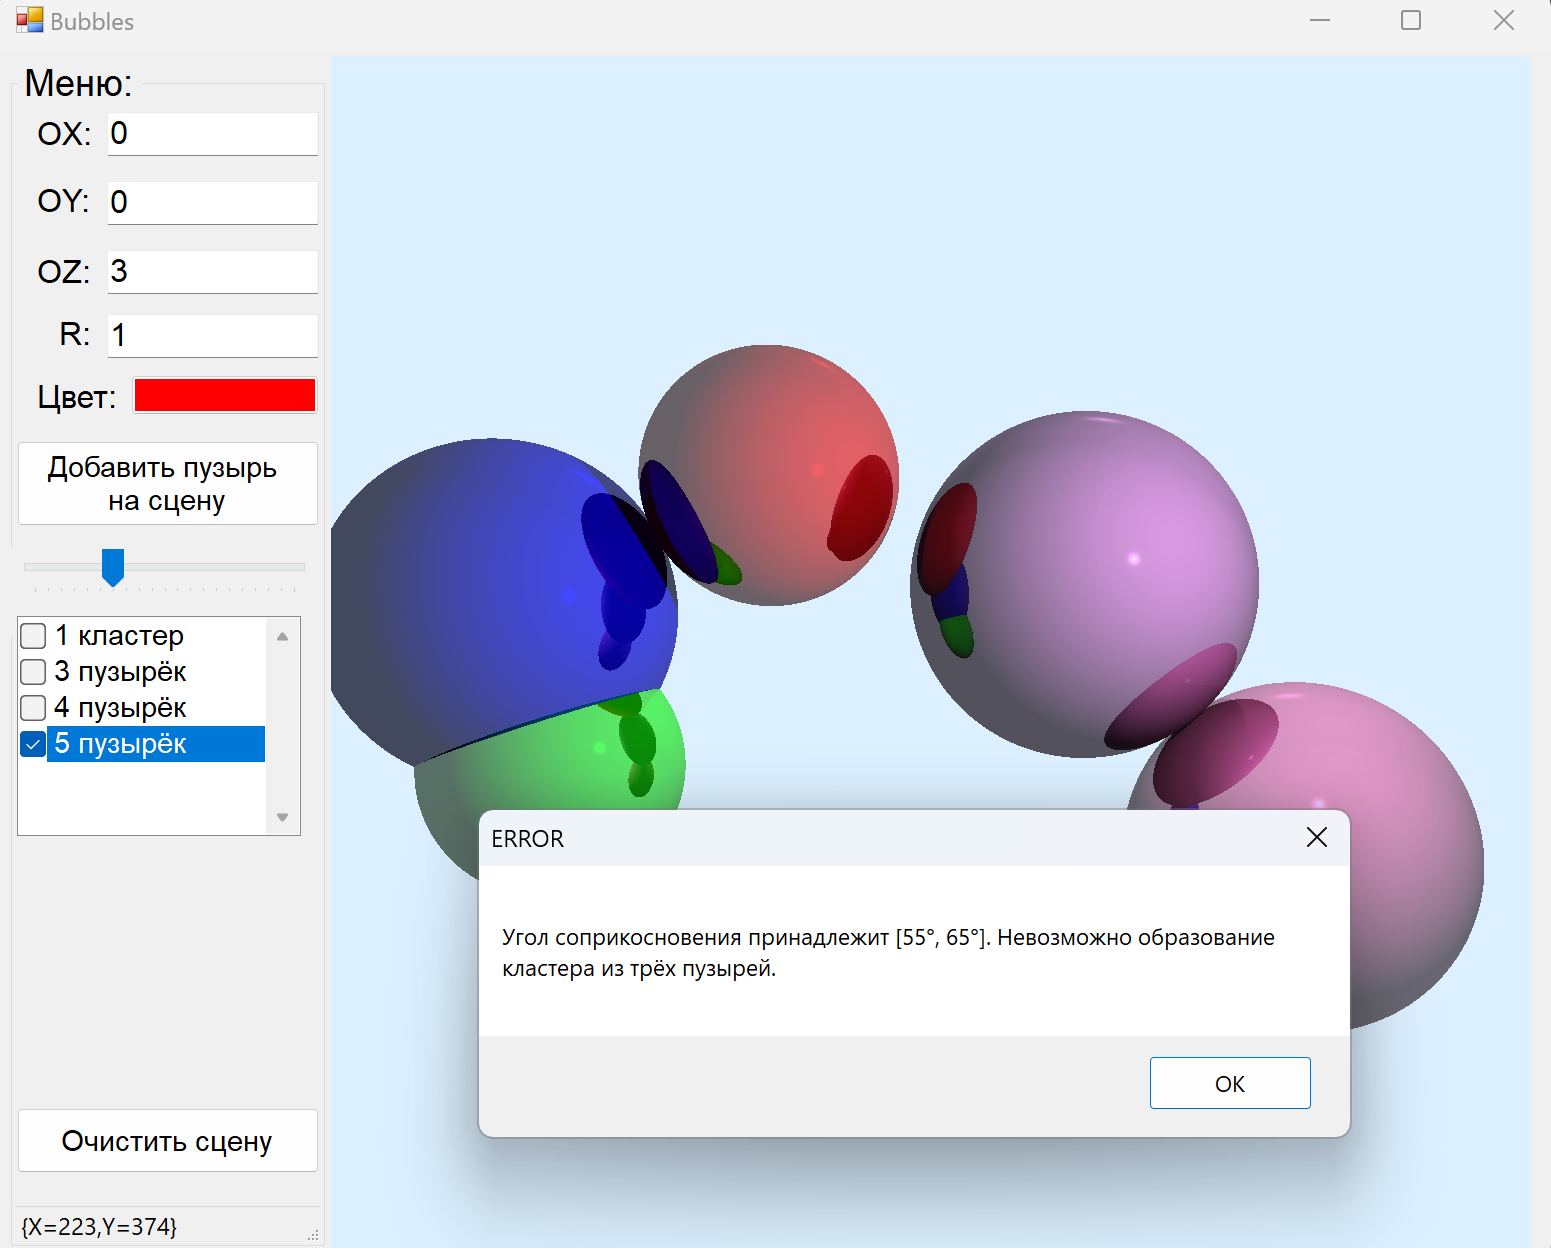
\includegraphics[width=\linewidth]{pictures/test6_2.png}
		\caption{После преобразования}
		\label{fig:6second}
	\end{subfigure}
	\caption{Тест №6: кластер из трёх пузырьков}
	\label{fig:test6}
\end{figure}

Все функциональные тесты пройдены успешно.